\documentclass[12pt]{article}
\usepackage[utf8]{inputenc}
\usepackage[T1]{fontenc}
\usepackage[english]{babel}
\usepackage[a4paper,margin=2.5cm]{geometry}
\usepackage{amsmath}
\usepackage{graphicx}
\usepackage{tikz}
\usepackage{listings}
\usepackage{xcolor}
\usepackage{booktabs}
\usetikzlibrary{arrows.meta,positioning}

\definecolor{codegray}{rgb}{0.95,0.95,0.95}
\lstset{
    basicstyle=\ttfamily\small,
    backgroundcolor=\color{codegray},
    frame=single,
    breaklines=true,
    columns=fullflexible
}

\title{Design of the Verification Testbench for \texttt{uart\_tx}}
\author{}
\date{}

\begin{document}

\maketitle

\section{Objective}

The goal of this testbench is to verify the UART transmitter module
\texttt{uart\_tx.v} located in \texttt{src/}. The assignment requires a
verification environment that takes into account a key timing fact: the input
clock is much faster than the serial baud rate. Because of that, the testbench
must validate the design in terms of clock cycles per UART bit, not in terms of
approximate real-number delays.

The final implementation is the self-checking file:

\begin{lstlisting}[language=Verilog]
tb/tb_uart_tx.v
\end{lstlisting}

\section{Relevant DUT Behavior}

The DUT is a basic 8N1 UART transmitter:

\begin{itemize}
    \item 1 start bit with value \texttt{0}
    \item 8 data bits transmitted LSB first
    \item 1 stop bit with value \texttt{1}
\end{itemize}

Its timing is controlled by:

\begin{lstlisting}[language=Verilog]
localparam CLOCKS_PER_BIT = CLK_FREQ / BAUD_RATE;
\end{lstlisting}

This means every transmitted bit must stay stable for exactly
\texttt{CLOCKS\_PER\_BIT} cycles. The DUT also has a few behavioral details that
directly shaped the testbench:

\begin{itemize}
    \item \texttt{rst\_n} is active low.
    \item \texttt{tx\_en} is sampled only in \texttt{s\_IDLE}.
    \item The start bit appears one clock after request acceptance.
    \item \texttt{tx\_busy} is a registered signal, not a pure decode of the FSM state.
    \item A short overlapping request while busy is ignored.
    \item A held-high \texttt{tx\_en} can be legally accepted again when the DUT returns to \texttt{s\_IDLE}.
\end{itemize}

The last two points are easy to confuse, so the testbench treats them as two
different corner cases.

\section{Why the Testbench Uses Reduced Parameters}

The RTL default parameters are:

\begin{itemize}
    \item \texttt{CLK\_FREQ = 27\_000\_000}
    \item \texttt{BAUD\_RATE = 115200}
    \item \texttt{CLOCKS\_PER\_BIT = 234}
\end{itemize}

Those values are correct, but they are slower to simulate. To keep the same
verification idea while reducing runtime, the implemented testbench instantiates
the DUT with:

\begin{lstlisting}[language=Verilog]
localparam integer CLK_FREQ       = 100_000;
localparam integer BAUD_RATE      = 1_000;
localparam integer CLOCKS_PER_BIT = CLK_FREQ / BAUD_RATE;
\end{lstlisting}

That gives:

\[
\texttt{CLOCKS\_PER\_BIT} = 100
\]

The important point is that the clock is still two orders of magnitude faster
than the baud rate, so the assignment's timing condition is preserved. The
testbench therefore remains realistic while running faster.

\section{General Architecture of the Testbench}

The testbench is self-checking and is organized around a small set of reusable
tasks.

\begin{figure}[h!]
\centering
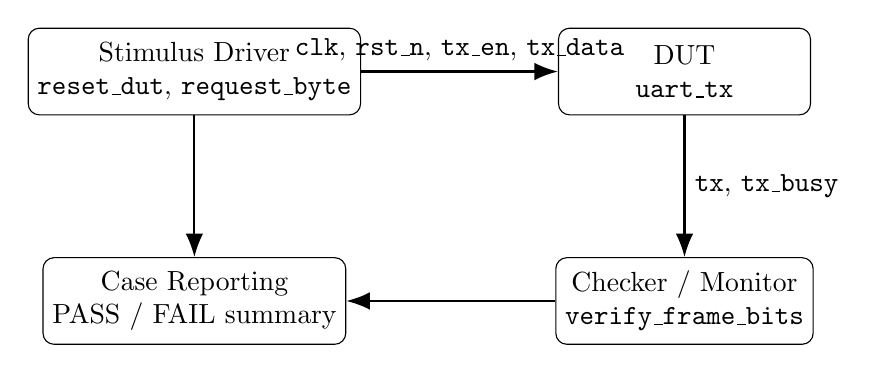
\begin{tikzpicture}[
    box/.style={draw, rounded corners, minimum width=3.2cm, minimum height=1.1cm, align=center},
    arrow/.style={-{Latex[length=3mm]}, thick}
]
    \node[box] (drv) {Stimulus Driver\\\texttt{reset\_dut}, \texttt{request\_byte}};
    \node[box, right=2.5cm of drv] (dut) {DUT\\\texttt{uart\_tx}};
    \node[box, below=1.8cm of dut] (chk) {Checker / Monitor\\\texttt{verify\_frame\_bits}};
    \node[box, below=1.8cm of drv] (rep) {Case Reporting\\PASS / FAIL summary};

    \draw[arrow] (drv) -- node[above] {\texttt{clk}, \texttt{rst\_n}, \texttt{tx\_en}, \texttt{tx\_data}} (dut);
    \draw[arrow] (dut) -- node[right] {\texttt{tx}, \texttt{tx\_busy}} (chk);
    \draw[arrow] (chk) -- (rep);
    \draw[arrow] (drv) -- (rep);
\end{tikzpicture}
\caption{High-level structure of the implemented UART TX testbench.}
\end{figure}

The main building blocks are:

\begin{itemize}
    \item a clock generator,
    \item a reset task,
    \item a normal one-cycle request driver,
    \item a short overlapping pulse driver,
    \item a frame checker based on cycle windows,
    \item and a case-by-case PASS/FAIL report.
\end{itemize}

\section{Why the Checks Are Cycle-Based}

Because the DUT is synchronous, the correct verification reference is the clock.
The testbench does not try to approximate UART timing with real-valued delays.
Instead, it checks that:

\begin{itemize}
    \item the start bit begins at the correct clock,
    \item every bit lasts exactly \texttt{CLOCKS\_PER\_BIT} cycles,
    \item data is transmitted LSB first,
    \item and \texttt{tx\_busy} stays asserted during the active frame.
\end{itemize}

The key checker is a cycle-window task:

\begin{lstlisting}[language=Verilog]
task check_bit_window;
    input expected_value;
    input integer bit_kind;
    input integer data_index;
    integer k;
    begin
        for (k = 0; k < CLOCKS_PER_BIT; k = k + 1) begin
            if (tx !== expected_value) begin
                ...
            end
            if (tx_busy !== 1'b1) begin
                ...
            end
            if (k != CLOCKS_PER_BIT - 1) begin
                @(posedge clk);
                #1;
            end
        end
    end
endtask
\end{lstlisting}

The small \texttt{\#1} delay is intentional. The DUT updates \texttt{tx} and
\texttt{tx\_busy} with nonblocking assignments on \texttt{posedge clk}, so the
testbench samples after the edge has settled. This avoids false failures caused
by checking the old value in the same simulation time slot.

\section{Driver Strategy}

Two different request styles are used in the testbench.

\subsection*{Normal Request}

The default task applies a one-cycle \texttt{tx\_en} pulse only when the DUT is
idle:

\begin{lstlisting}[language=Verilog]
task request_byte;
    input [7:0] data_byte;
    output integer accepted_cycle;
    begin
        wait_for_idle();
        @(negedge clk);
        tx_data = data_byte;
        tx_en   = 1'b1;
        @(posedge clk);
        #1;
        accepted_cycle = cycle_count;
        ...
        @(negedge clk);
        tx_en = 1'b0;
    end
endtask
\end{lstlisting}

This driver is used for nominal traffic and for back-to-back legal transfers.

\subsection*{Special Request Patterns}

Two special patterns are used for corner cases:

\begin{itemize}
    \item a short overlapping pulse while the DUT is busy,
    \item a held-high \texttt{tx\_en} that remains asserted until the DUT returns to \texttt{s\_IDLE}.
\end{itemize}

They are both important because the DUT is level-sensitive in \texttt{s\_IDLE},
not edge-sensitive.

\section{Tested Cases}

The implemented testbench explicitly highlights and runs the following seven
cases.

\begin{center}
\begin{tabular}{@{}ll@{}}
\toprule
\textbf{Case} & \textbf{Purpose} \\
\midrule
1 & Reset behavior \\
2 & Single nominal transmission \\
3 & Pattern sensitivity and LSB-first ordering \\
4 & Data capture vs later \texttt{tx\_data} changes \\
5 & Short overlapping request while busy is ignored \\
6 & Held-high \texttt{tx\_en} causes legal immediate reacceptance \\
7 & Back-to-back legal transmissions \\
\bottomrule
\end{tabular}
\end{center}

\subsection*{1. Reset Behavior}

This case checks that:

\begin{itemize}
    \item \texttt{tx} immediately goes high during reset,
    \item \texttt{tx\_busy} goes low during reset,
    \item and the DUT remains idle after reset release.
\end{itemize}

\subsection*{2. Single Nominal Transmission}

A non-trivial byte, \texttt{8'hA5}, is transmitted and the testbench verifies:

\begin{itemize}
    \item request acceptance,
    \item one-cycle delay before the start bit,
    \item correct frame ordering,
    \item exact bit duration,
    \item and return to idle after the stop bit.
\end{itemize}

\subsection*{3. Pattern Sensitivity and Bit Ordering}

Several patterns are sent:

\begin{itemize}
    \item \texttt{8'h00}
    \item \texttt{8'hFF}
    \item \texttt{8'h55}
    \item \texttt{8'hAA}
    \item \texttt{8'h3C}
\end{itemize}

These patterns give confidence against:

\begin{itemize}
    \item stuck-at faults,
    \item wrong bit order,
    \item bad serialization,
    \item and missing transitions on the serial output.
\end{itemize}

\subsection*{4. Data Capture Versus Later Input Changes}

The DUT stores the requested byte in \texttt{tx\_data\_reg} when the transfer is
accepted. To verify that behavior, the testbench changes \texttt{tx\_data}
during an active frame and checks that the transmitted byte still matches the
original accepted value.

\subsection*{5. Short Overlapping Request While Busy}

This case applies a one-cycle \texttt{tx\_en} pulse while a frame is already in
progress, then removes it before the DUT returns to idle. The testbench checks
that:

\begin{itemize}
    \item the active frame is not corrupted,
    \item no extra transfer is accepted,
    \item and \texttt{tx\_busy} remains consistent.
\end{itemize}

\subsection*{6. Held-High \texttt{tx\_en}}

This case is intentionally separate from the previous one. If \texttt{tx\_en}
stays high until the DUT returns to \texttt{s\_IDLE}, the RTL may legally accept
another transfer immediately. The testbench treats this as expected behavior and
checks that the second frame starts correctly.

\subsection*{7. Back-to-Back Legal Transmissions}

Two valid requests are applied in sequence, each when the DUT is idle. This
verifies clean frame termination, correct re-entry into idle, and correct
acceptance of the next transfer.

\section{Validation Command}

The testbench was validated using the repository's verification builder:

\begin{lstlisting}[language=bash]
./VERIFICATION/builder-verification.sh -r uart-verification -x
\end{lstlisting}

The build generated:

\begin{itemize}
    \item the simulation binary in \texttt{build/},
    \item the waveform file \texttt{build/tb\_uart\_tx.vcd},
    \item and a final PASS result from the self-checking testbench.
\end{itemize}

\section{Final Result}

The final implemented testbench executed:

\begin{itemize}
    \item 7 highlighted verification cases,
    \item 24106 individual checks,
    \item and 0 failures.
\end{itemize}

This confirms that the UART transmitter satisfies the intended behavior under
reset, nominal transfers, timing-sensitive frame checking, capture semantics,
busy overlap handling, held-high request semantics, and back-to-back operation.

\section{Conclusion}

The final verification strategy is intentionally cycle-accurate, self-checking,
and compatible with the repository flow. The design of \texttt{tb/tb\_uart\_tx.v}
is driven by the real behavior of the DUT:

\begin{itemize}
    \item synchronous updates on clock edges,
    \item bit timing defined by \texttt{CLOCKS\_PER\_BIT},
    \item registered \texttt{tx\_busy},
    \item and level-sensitive request handling in \texttt{s\_IDLE}.
\end{itemize}

Because of that, the testbench does more than just send bytes and look at the
waveform. It actively checks timing windows, handshake semantics, capture
behavior, and edge cases that are easy to misinterpret if they are not tested
separately.

\end{document}
